\chapter{目前仍存在的bug与解决思路}

\section{硬件方面}

由于今年的开发板从 2k500 换成了 2k1000 且其\textbf{标称型号与实际型号相同性存疑},我们在上板期间遇到了许多问题,这里不再详细列举,下面给出网上找到的 2k1000 开发板与实物存在的区别

\begin{figure}[htbp]
	\centering
	\begin{minipage}{0.49\linewidth}
		\centering
		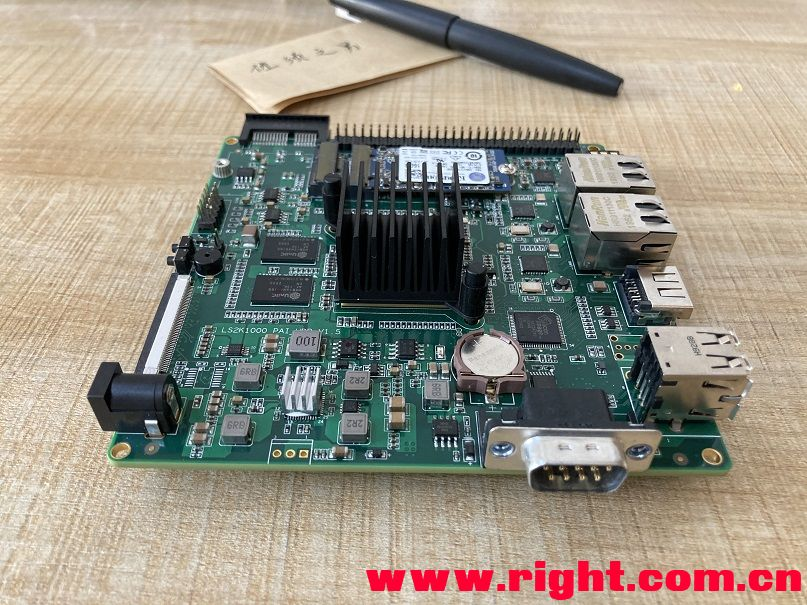
\includegraphics[width=0.9\linewidth]{figs/2k1000pi.jpg}
		\caption{网上找到的 2k1000 开发板}
		\label{Board-Internet}
	\end{minipage}
	\begin{minipage}{0.49\linewidth}
		\centering
		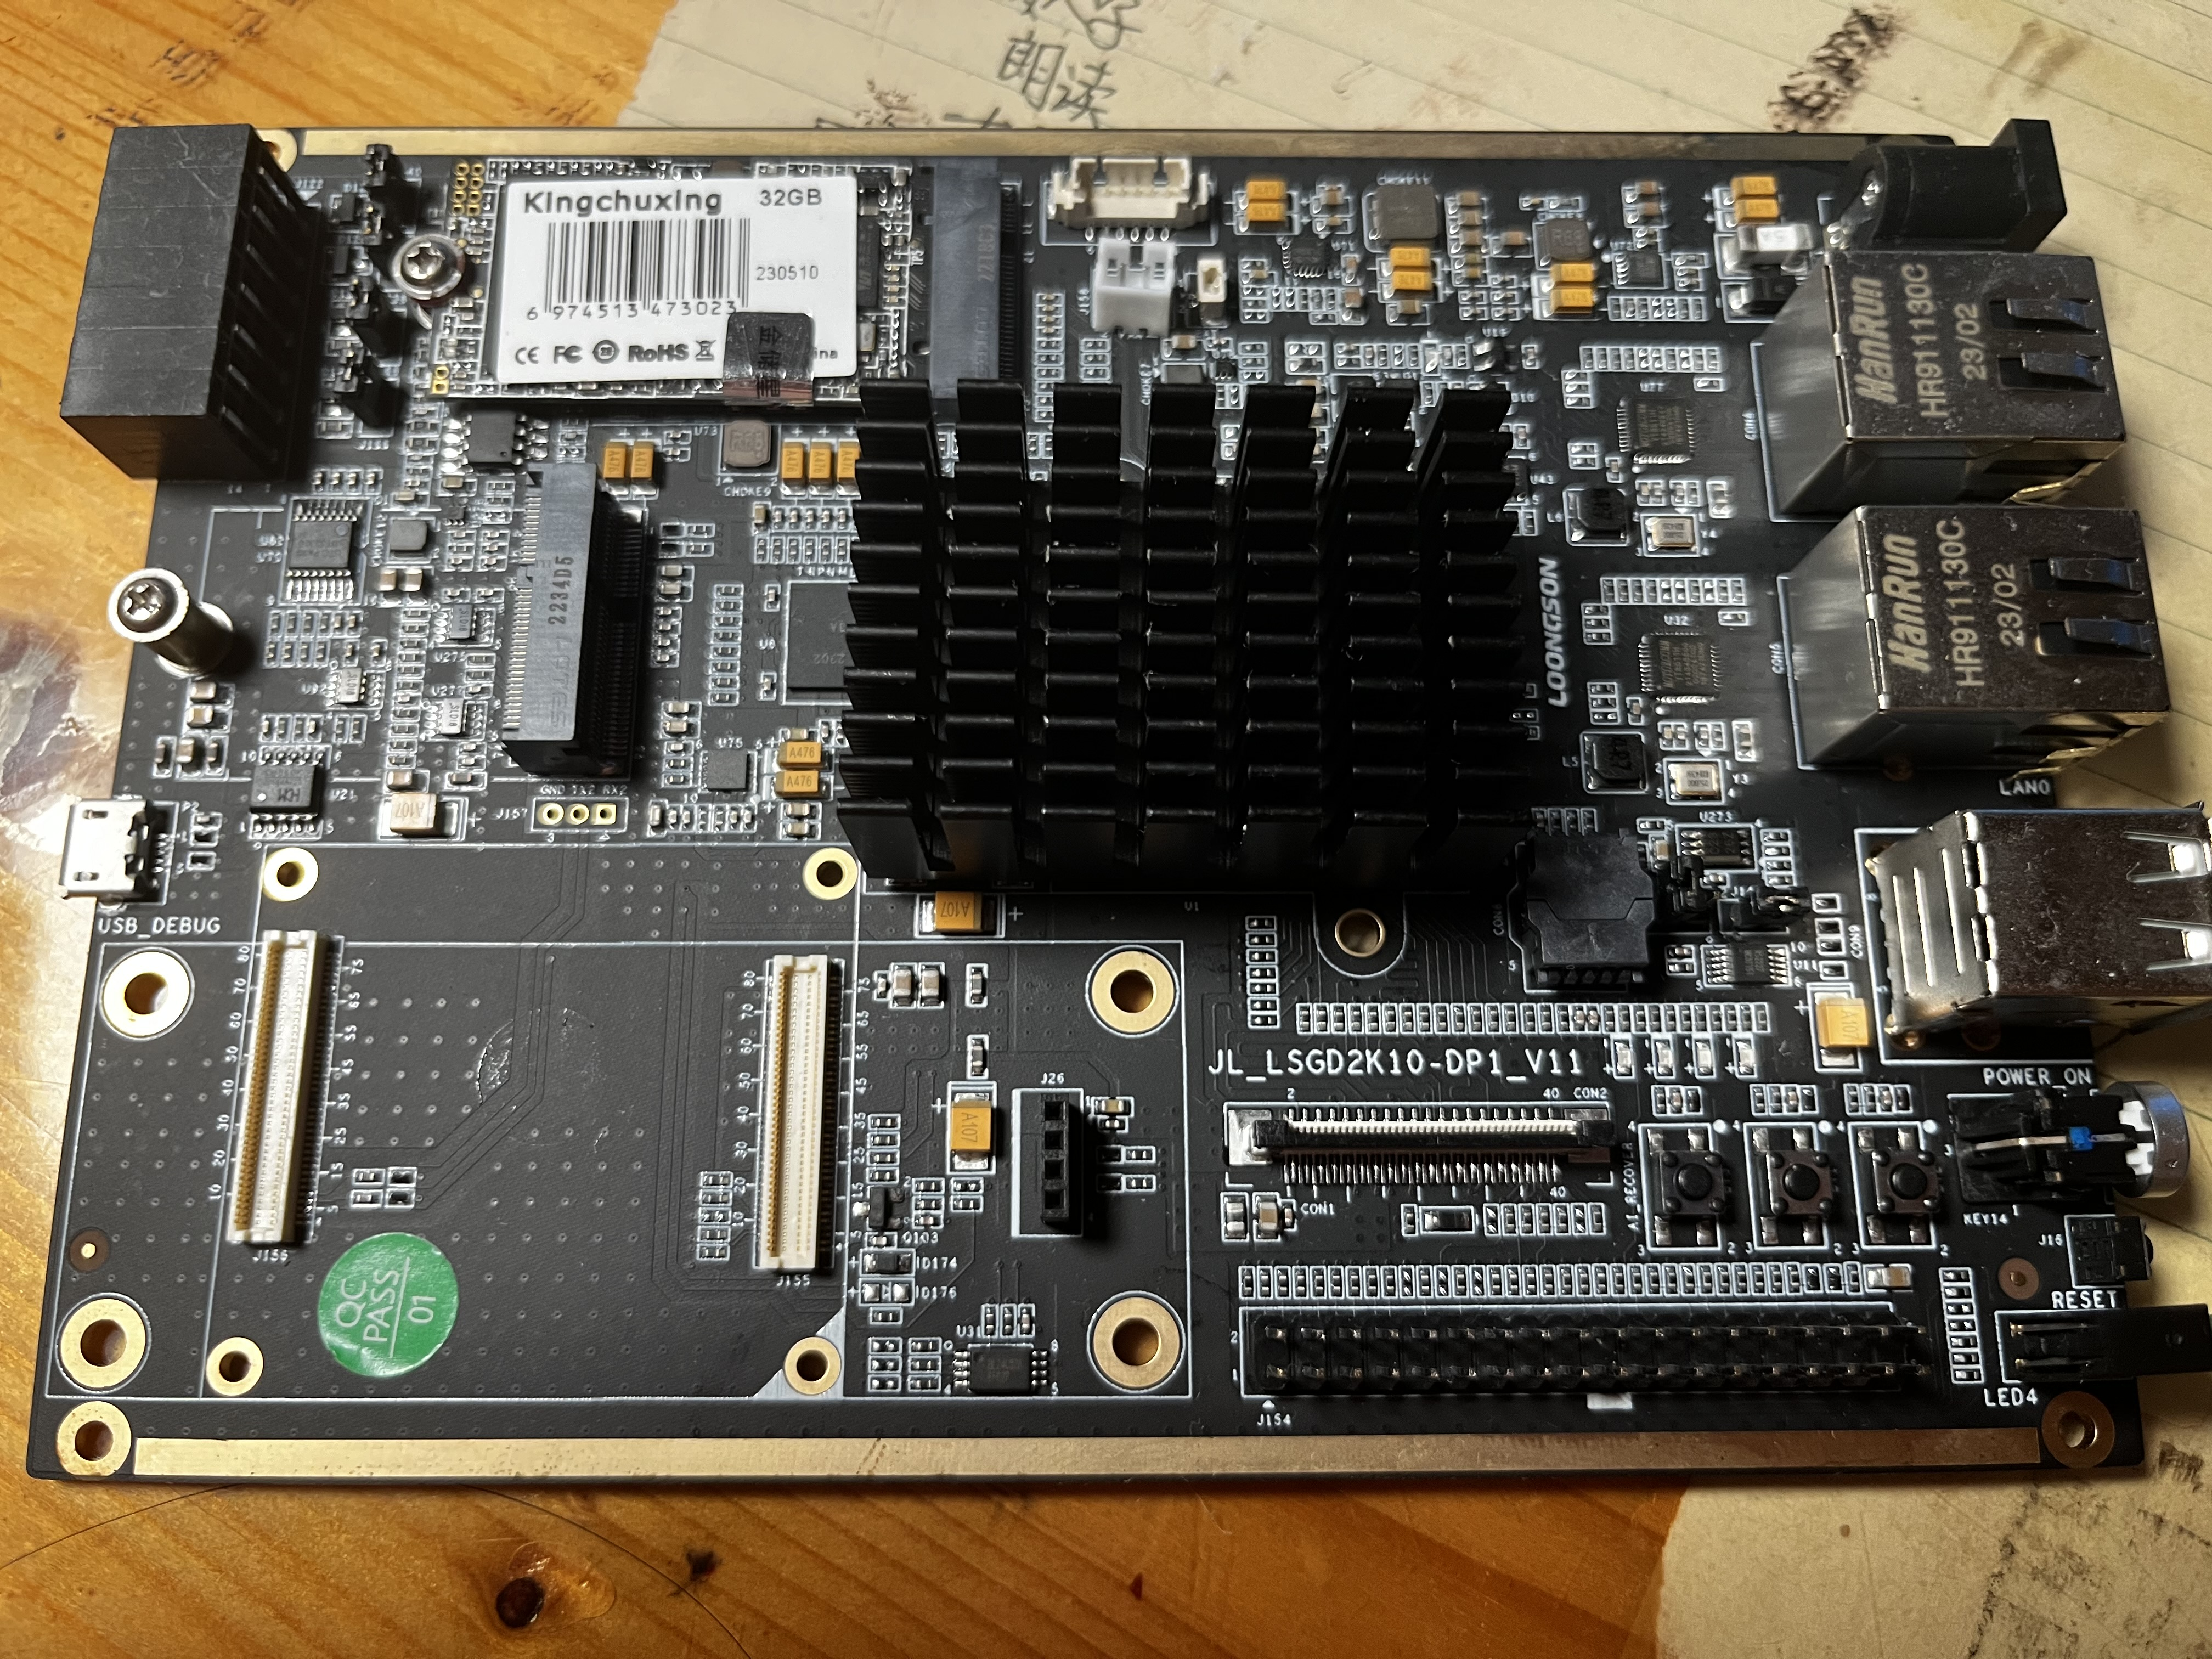
\includegraphics[width=0.9\linewidth]{figs/2k10dp1v11.jpg}
		\caption{实物}
		\label{Board-RealEstate}
	\end{minipage}
\end{figure}

下表中给出我们在 Debug 期间找到的不同之处

\begin{table}[htbp]
	\begin{center}
		\begin{tabular}{|c|c|c|c|c|c|}
			\hline
			& NAND & SATA接口 & 串口 & uboot系统\\
			\hline
			\hline
			网传 & 有 & 有 & 有 & \textbf{存在差异} \\
			\hline
			实物 & 无 & 无 & 无 & \textbf{存在差异} \\
			\hline
		\end{tabular}
		\caption{2k1000 实际不同之处}
	\end{center}
\end{table}

即便如此,我们得到的 2k1000 开发板的 u-boot 系统仍然不尽人意,以下是我们找到的几个问题

\begin{enumerate}
	\item \textit{NAND 芯片缺失问题:}我们发现,开发板在子系统中搭载了 NAND-Subsystem ,但利用指令扫描设备时并未发现 NAND 芯片,这令我们困扰,在仔细检查过开发板后,我们发现开发板其实并未搭载 NAND 芯片.
		  \begin{figure}[htbp]
			\centering
			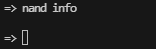
\includegraphics[width=0.5\linewidth]{figs/nand设备情况.png}
			\caption{nand设备情况}
			\label{nand设备情况}
		  \end{figure}
	\item \textit{MMC 子系统缺失问题:}不仅如此,我们在后续进行烧录操作时,发现本开发板搭载的 u-boot 系统甚至没有搭载 MMC 子系统,这表示这我们无法对上面的 SSD 进行操作, \textbf{这直接导致了下面存在的问题}.
\end{enumerate}

\subsection{上板期间遇到的问题I —— 无法烧录}

由于复赛期间我们强制要求使用 mkfs_ext4 进行镜像文件系统的制作,并强制将测例封装进文件系统,我们在上板测试时发现了如下问题

\subsubsection{现象}

我们在正常烧录内核时,会在初始化  报Panicked,具体现象与代码如下:

\begin{figure}[htbp]
	\centering
	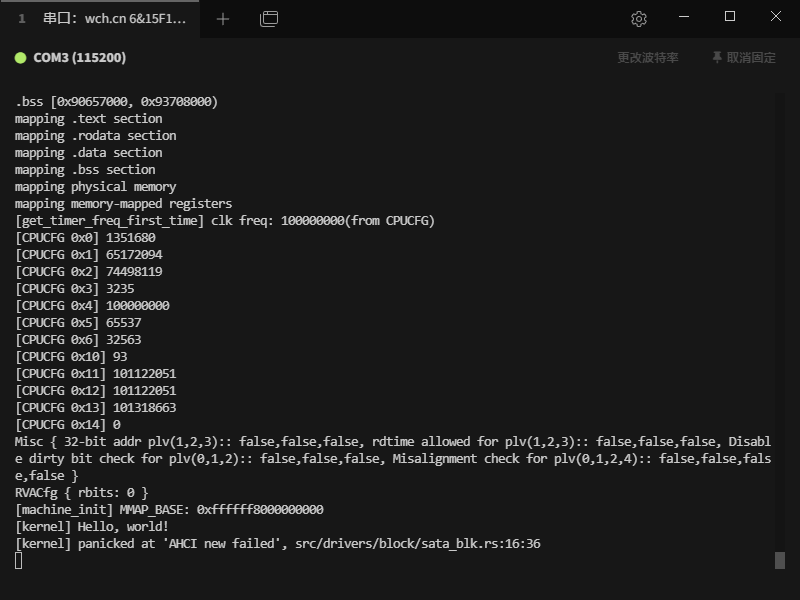
\includegraphics[width=0.5\linewidth]{figs/bug.png}
	\caption{报错信息}
	\label{information of bug}
\end{figure}

经过分析,我们认为,在这里 Panicked 是因为内核在初始化时没有找到文件系统,\textbf{所以产生了 Block 相关问题},我们的文件系统在 QEMU 中是提前使用指令挂载至虚拟硬盘之中的

\begin{figure}[htbp]
	\centering
	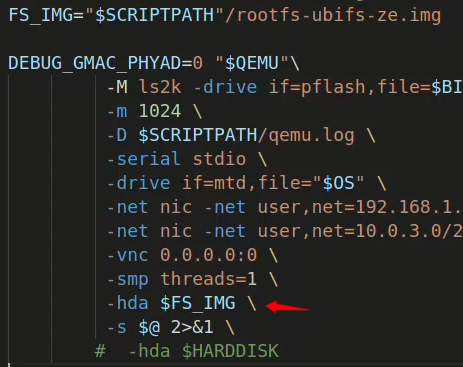
\includegraphics[width=0.5\linewidth]{figs/hda.png}
	\caption{QEMU 中挂载源码}
	\label{information of bug}
\end{figure}

\subsubsection{解决方法}

于是我们试图通过某种方式绕过这些问题

\begin{enumerate}
	\item \textit{通过 USB 启动:}我们在发现无法针对板上存储设备进行操作之后,试图利用 USB 启动方式绕过 u-boot 的缺陷
	\begin{enumerate}
		\item \textbf{挂载方式:}通过将 USB 设备作为硬盘\footnote{参考例子:https://www.cnblogs.com/nhdlb/p/14726431.html},将引导区域与内核区域放在一起以绕过这个缺陷
		\item \textbf{结果:}内核无法识别两个分区的( A 分区挂载引导与内核; B 分区挂载文件系统镜像) USB 启动硬盘
	\end{enumerate}
	\item \textit{刷入 PMON 系统:}
	\begin{enumerate}
		\item \textbf{PMON 系统简介:}
		\begin{enumerate}
			\item 龙芯平台计算机目前多采用 PMON 作为基本的输入输出系统
			\item PMON具有强大而丰富的功能,包括硬件初始化、操作系统引导和硬件测试、程序调式等功能
			\item 它提供多种加载操作系统的方式,可以从优盘、光盘、 tftp 服务器和硬盘等媒介加载;它提供对内存、串口、显示、网络、硬盘等的基础测试工具;此外,它还支持软件升级
		\end{enumerate}
	\end{enumerate}
\end{enumerate}